\documentclass{../lab}

\labacronym{ATM}
\labtitle{Atomic Physics}

%\newcommand{\VideoOpticalInstruments}{http://youtu.be/zUGBt5vc5FA}
%\newcommand{\EnergyLevelData}{http://physics111.lib.berkeley.edu/Physics111/Reprints/ATM/ATM_index.html}
%\newcommand{\Fabry-Perot}{http://physics111.lib.berkeley.edu/Physics111/Reprints/ATM/OCR\%20Burleigh\%20tech\%20memo\%20fabry\%20perots.pdf}
%\newcommand{\Ch.10:Diffraction}{http://physics111.lib.berkeley.edu/Physics111/Reprints/ATM/Optics\%20Hecht\%20&\%20Zajac/Ch.\%2010\%20diffraction.pdf}
%\newcommand{\AtomicSpectra\&AtomicStructure}{http://physics111.lib.berkeley.edu/Physics111/Reprints/ATM/02-2ndEd-Atomic_Spectra_and_Atomic_Structure.pdf}
%\newcommand{\Ch.18:HyperfineStructure}{http://physics111.lib.berkeley.edu/Physics111/Reprints/ATM/Introduction\%20to\%20Atomic\%20Harvey\%20E.\%20White/Ch.\%2018\%20hyperfine\%20structure_OCR.pdf}
%\newcommand{\AppendixI:ARCModelAM-505AtmosphericMonochromator}{http://experimentationlab.berkeley.edu/ATMAppendix1}
%\newcommand{\PhotomulitiplierTubesCh.9}{http://physics111.lib.berkeley.edu/Physics111/Reprints/Knoll-Radiation\%20Detection\%20&\%20Measurement/01-Radiation_Detection_and_Measurement_CH_09.pdf}
%\newcommand{\}{http://experimentationlab.berkeley.edu/sites/default/files/images/LLSimage019.gif}
%\newcommand{\Ch.14:InterferenceInvolvingMultipleReflections}{http://physics111.lib.berkeley.edu/Physics111/Reprints/ATM/04-Interference.pdf}

\begin{document}

\maketitle

\tableofcontents

\section{Atomic Physics Description (ATM)}

\begin{enumerate}
    \item \textbf{Note that there is NO eating or drinking in the 111-Lab anywhere, except in rooms 282 \& 286 LeConte on the bench with the BLUE stripe around it.} Thank you - the Staff.

\end{enumerate}

Atomic spectroscopy was the proving ground for Quantum Mechanics. In this lab you will observe the emission lines of mercury and hydrogen over the range 250 to 750 nm, using a diffraction-grating spectrometer. You will identify and measure the Balmer series of spectral lines in hydrogen, and then use the results to determine the energy levels and the value of the Rydberg constant. Mercury lines are used to calibrate the wavelength scale of the spectrometer.

In 1896 Peter Zeeman observed the broadening and polarization of spectral lines of sodium when the source was placed in a magnetic field. Since that time both the changes in the energy levels of an individual atom and the splitting of spectral lines in a magnetic field have carried the name Zeeman Effect.

After observing the principal spectral lines in hydrogen, you will go on to measure the Zeeman effect in a single spectral line of helium. A high voltage discharge tube filled with helium is placed between the poles of an electromagnet. Light from the lamp is analyzed with a Fabry-Perot interferometer. From your data you will calculate the magnitude of the Bohr magneton.

In addition to atomic physics and quantum mechanics, this lab emphasizes optics.

You need to be present for all parts of the experiment. You can't leave while the data are being recorded. If you know what you are doing and don't make any mistake, you can complete the data-taking in 4 days.

You will need to review (perhaps see for the first time) optics at the sophomore and junior levels. You may have had very little in formal classroom work about mirrors, lenses, spectrometers, diffraction gratings, and \href{http://experimentationlab.berkeley.edu/sites/default/files/ATM/Etalons\_TechNote-3pages.pdf}{\textbf{Fabry-Perot interferometers}}. You will need to integrate practical knowledge about spectra, spectroscopic terminology, and energy level diagrams, with the more abstract quantum theory of atoms. None of the subjects is difficult, but each requires time. Your study will be a good review for parts of the advanced GRE.

\begin{enumerate}
    \item Pre-requisites: Physics 137AB

    \item Days Allotted for the Experiment: 6

\end{enumerate}

This lab will be graded 40\% on theory, 40\% on technique, and 20\% on analysis. For more information, see the \href{\AdvancedLabSyllabus}{\textbf{Advanced Lab Syllabus.}}

Comments: \Feedback

\pagebreak 

\section{The Atomic Physics Experiment Photos}

\begin{figure}[H]
\captionsetup{justification=centering}
\minipage{0.32\textwidth}
  \href{http://experimentationlab.berkeley.edu/sites/default/files/images/ATM-mono-Grating_3500-Lg.jpg}{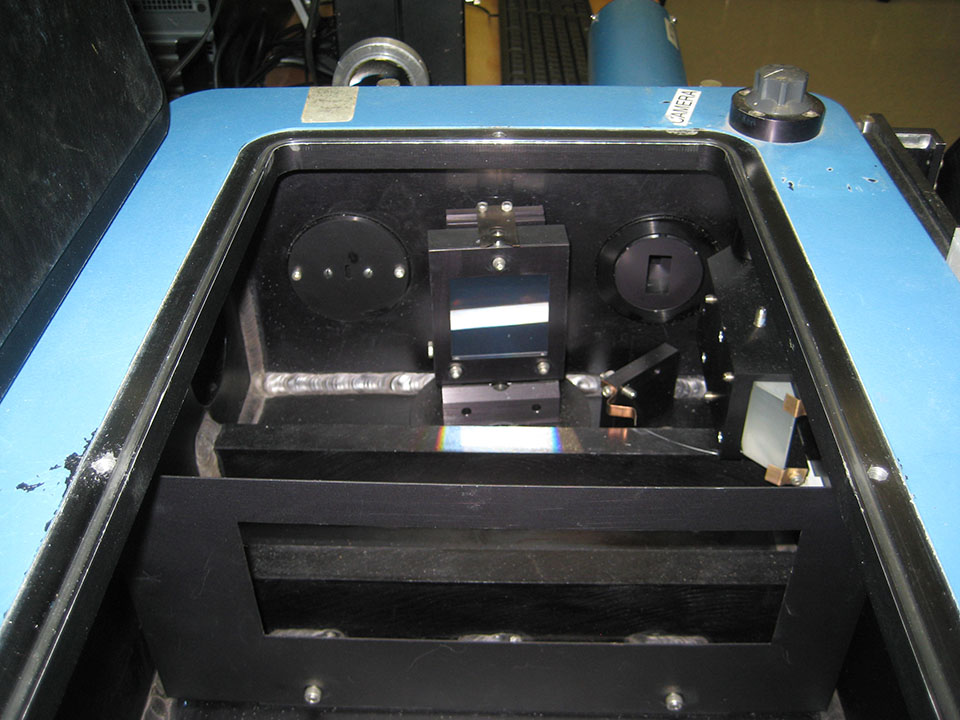
\includegraphics[height=120pt,keepaspectratio]{images/ATM-mono-Grating_3500-Lg.jpg}}
  \caption{Grating, Entrance, and \\ Exit Slit Interior View \\ \href{http://experimentationlab.berkeley.edu/sites/default/files/images/ATM-mono-Grating_3500-Lg.jpg}{Click here to see larger picture}}
  \label{fig:MonochrometerInteriorSide}
\endminipage\hfill
\minipage{0.32\textwidth}
  \href{http://experimentationlab.berkeley.edu/sites/default/files/images/ATM-mono-In-Topview_3501-Lg.jpg}{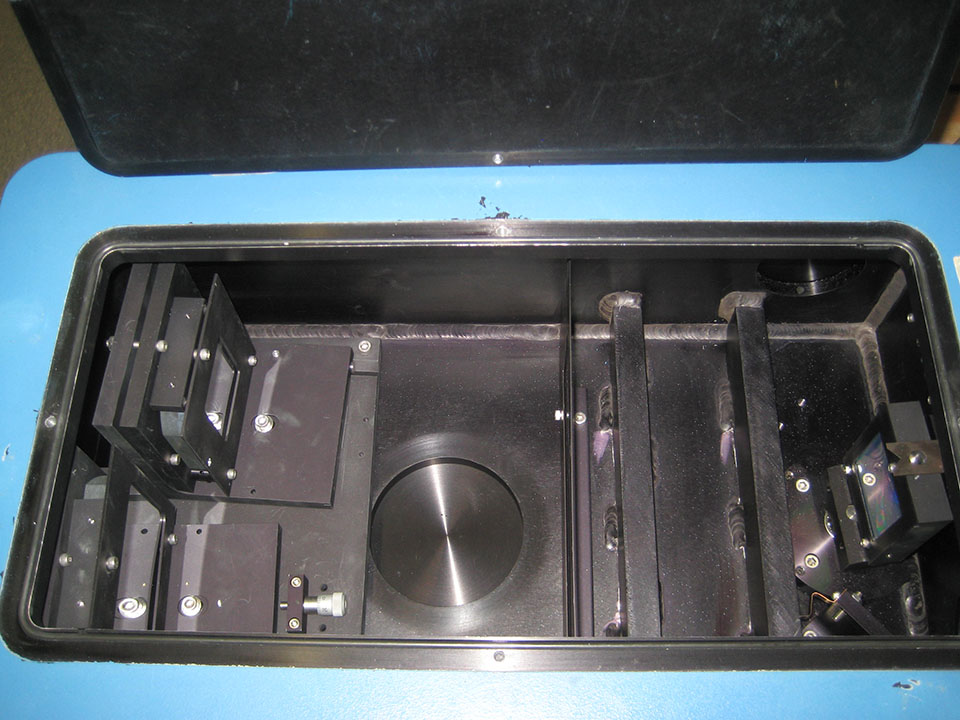
\includegraphics[height=120pt,keepaspectratio]{images/ATM-mono-In-Topview_3501-Lg.jpg}}
  \caption{Monochrometer \\ Interior Top View\\ \href{http://experimentationlab.berkeley.edu/sites/default/files/images/ATM-mono-In-Topview_3501-Lg.jpg}{Click here to see larger picture}}\label{fig:MonochrometerInteriorTop}
\endminipage \hfill
\minipage{0.30\textwidth}
  \href{http://experimentationlab.berkeley.edu/sites/default/files/images/ATM-mono-In-Mirrors_3499-Lg.jpg}{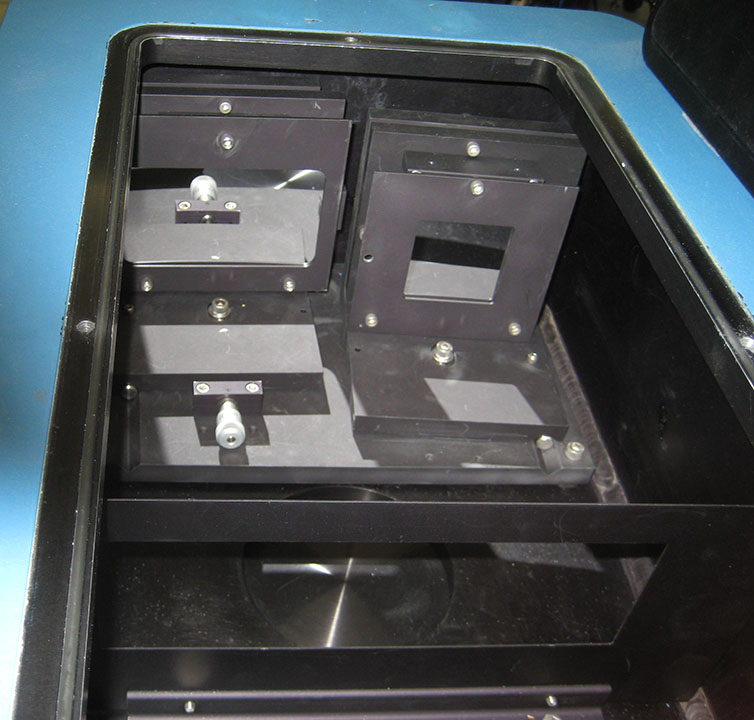
\includegraphics[height=120pt,keepaspectratio]{images/ATM-mono-In-Mirrors_3499-Lg.jpg}}
  \caption{Monochrometer \\ Interior Mirror View \\ \href{http://experimentationlab.berkeley.edu/sites/default/files/images/ATM-mono-In-Mirrors_3499-Lg.jpg}{Click here to see larger picture}}\label{fig:Multiplet}
\endminipage
\end{figure}

\begin{figure}[H]
\captionsetup{justification=centering}
\minipage{0.49\textwidth}
  \href{http://experimentationlab.berkeley.edu/sites/default/files/images/ATM_Balmer_3490-Crop-Lg.jpg}{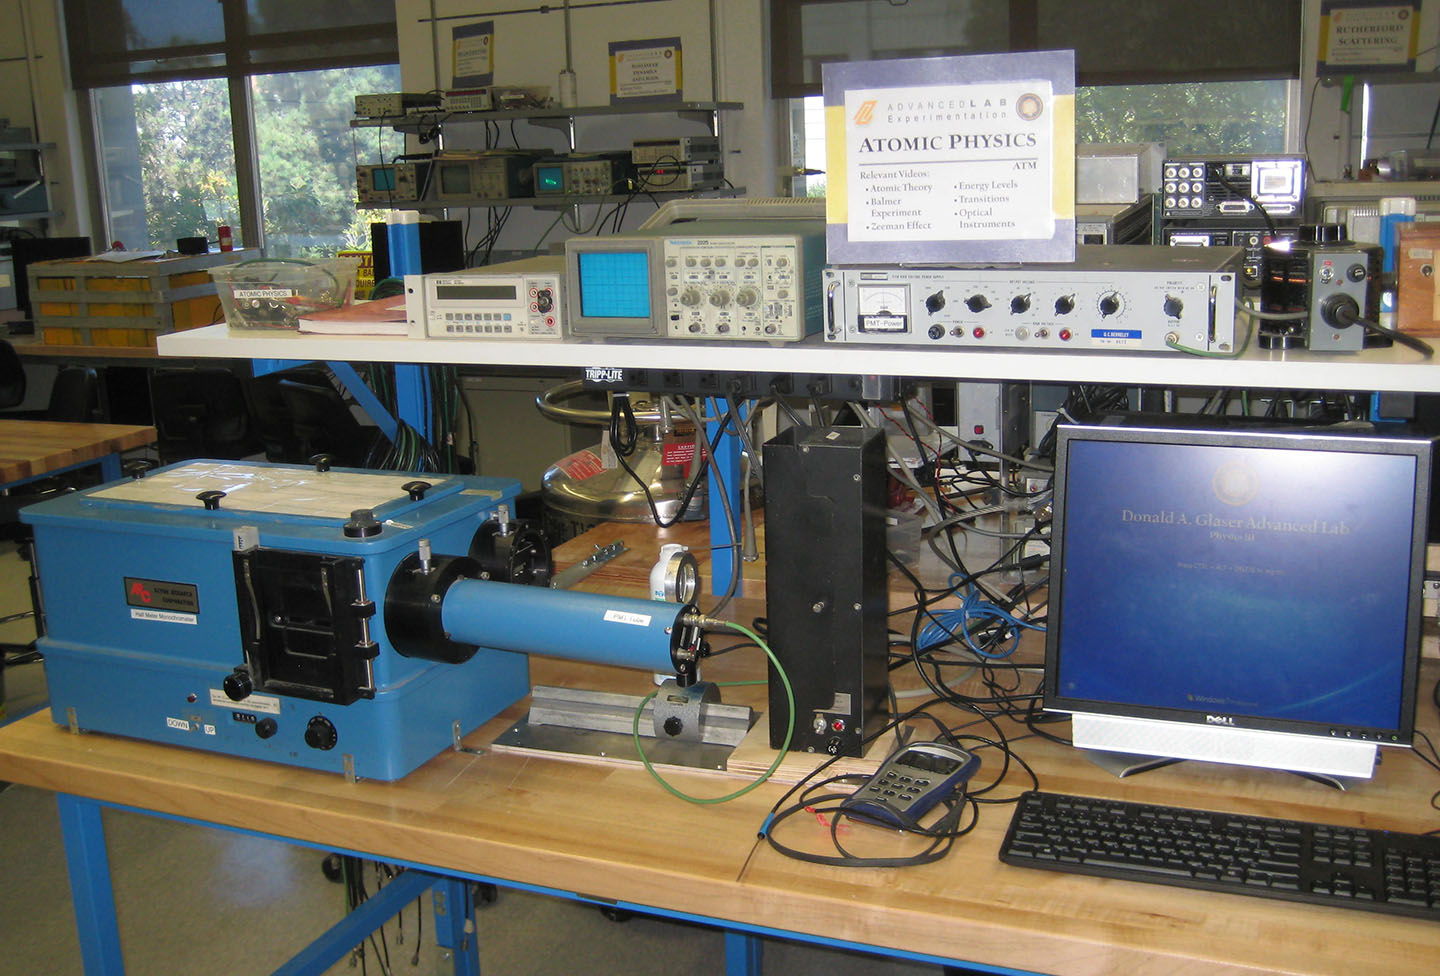
\includegraphics[height=160pt,keepaspectratio]{images/ATM_Balmer_3490-Crop-Lg.jpg}}
  \caption{Balmer Setup with the Computer \\ \href{http://experimentationlab.berkeley.edu/sites/default/files/images/ATM_Balmer_3490-Crop-Lg.jpg}{Click here to see larger picture}}
  \label{fig:BalmerApparatus}
\endminipage\hfill
\minipage{0.49\textwidth}
  \href{http://experimentationlab.berkeley.edu/sites/default/files/images/ATM_ZeemanSetup_3492-Crop-Lg.jpg}{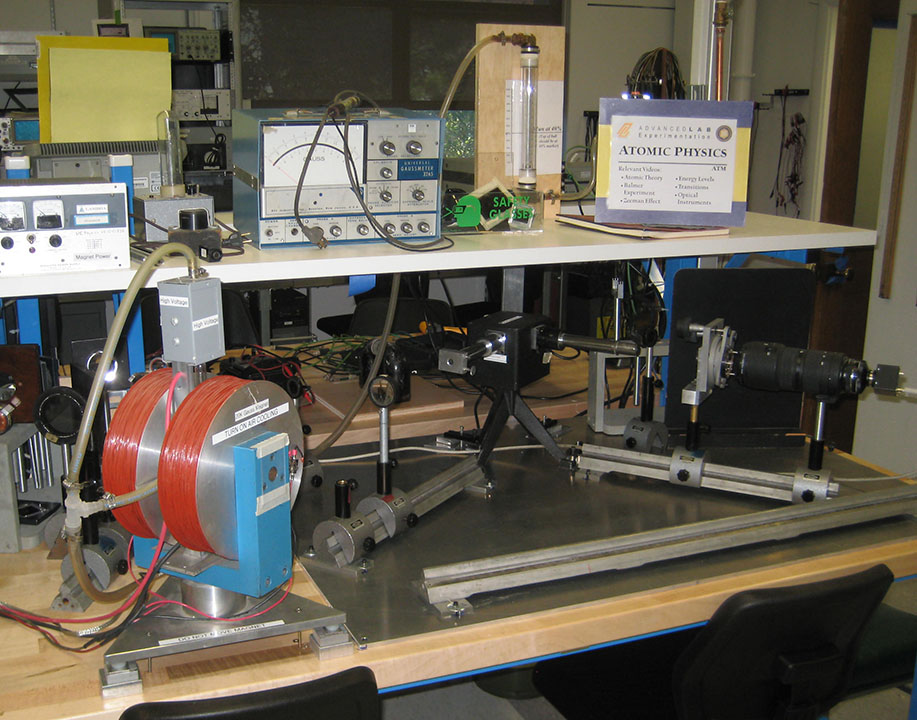
\includegraphics[height=160pt,keepaspectratio]{images/ATM_ZeemanSetup_3492-Crop-Lg.jpg}}
  \caption{Zeeman Effect Apparatus \\
  \href{http://experimentationlab.berkeley.edu/sites/default/files/images/ATM_ZeemanSetup_3492-Crop-Lg.jpg}{Click here to see larger picture}}
  \label{fig:ZeemanApparatus}
\endminipage

\end{figure}

\begin{figure}[H]
\captionsetup{justification=centering}
\minipage{0.35\textwidth}
\centering
  \href{http://experimentationlab.berkeley.edu/sites/default/files/images/Atm_5.jpg}{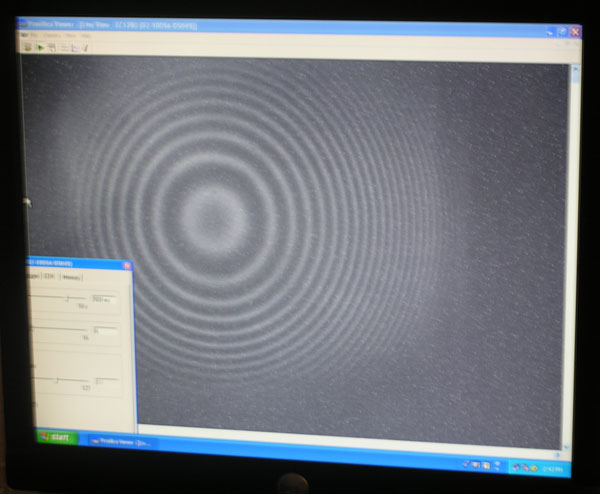
\includegraphics[height=120pt,keepaspectratio]{images/Atm_5.jpg}}
  \caption{Captured Image from Fabry-Perot Interferometer \\
  \href{http://experimentationlab.berkeley.edu/sites/default/files/images/Atm_5.jpg}{Click here to see larger picture}}
  \label{fig:ImagedFringes}
\endminipage\hfill
\minipage{0.34\textwidth}
\centering
  \href{http://experimentationlab.berkeley.edu/sites/default/files/images/Atm1image003.png}{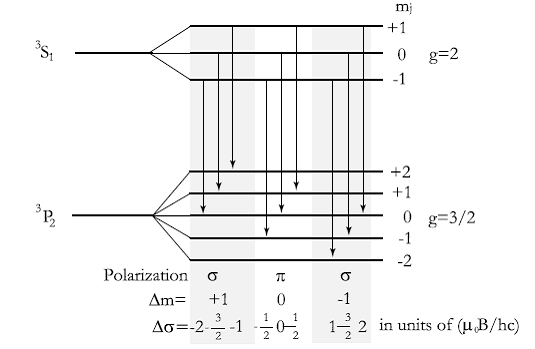
\includegraphics[height=120pt,keepaspectratio]{images/Atm1image003.png}}
  \caption{Zeeman Multiplet Splitting \\
  \href{http://experimentationlab.berkeley.edu/sites/default/files/images/Atm1image003.png}{Click here to see larger picture}}
  \label{fig:SafetyGlasses}
\endminipage\hfill
\minipage{0.30\textwidth}
\centering
  \href{http://experimentationlab.berkeley.edu/sites/default/files/upimages/3_eye-wear-face.jpg}{
\includegraphics[height=130pt,keepaspectratio]{images/3_eye-wear-face.jpg}}
  \caption{\textbf{Wear Your \\ Safety Glasses}}
\endminipage
\end{figure}

\section{Before the 1st day of Lab}

\signatures \hyperlink{Preparation}{ 1} \hyperlink{Peak Finding}{ 2} \hyperlink{Additional Questions}{ 3} \hyperlink{Zeeman Picture}{ 4} \hyperlink{Zeeman Splitting}{ 5}

\begin{enumerate}
    \item \emph{\textbf{Note: In order to view the private Youtube videos hosted by the university, you must be signed into your berkeley.edu Google account.}} \\
    View the three videos \href{http://youtu.be/iJ\_4ygOaE7A}{\textbf{Atomic Theory Only Video}} (Great Introduction to ATM, 37 minutes long), \href{http://youtu.be/M41IKkUAG-A}{\textbf{Video on Balmer Series Part-1}} (20 minutes long), and the \href{http://youtu.be/-l2chO5SLew}{\textbf{Video on Zeeman Effect Part-2}} (30 minutes long).

    %\item \emph{Checkpoints are examination points where you must STOP and get a GSI or professor to verify your understanding and/or verify proper experimental setup. You cannot skip the checkpoints, as there is a \sig that must be scanned in with your lab report. Print out the checkpoints page now and look it over.}

    %\item Complete the \href{http://experimentationlab.berkeley.edu/ATMPreLab}{\textbf{ATM Pre Lab and Evaluation}} sheets (see number 4 below). Print, fill out the answers, and turn in with your report. The pre-Lab must be printed separately. Discuss the experiment and pre-lab questions and answers with any faculty member or GSI and get it signed off by that faculty member or GSI. Turn in the signed pre-lab sheet with your lab report.

    \item View the optics tutorial article (7pgs), a great review of the principles of optics, \href{http://experimentationlab.berkeley.edu/sites/default/files/QIE/fundamental-Optics.pdf}{\textbf{Fundamentals of Optics Tutorial}}\textbf{ }and the \href{http://youtu.be/zUGBt5vc5FA}{\textbf{Light and Optical Instruments Video}}\textbf{ }(Good introduction to light and optics, 50 minutes long), \href{http://youtu.be/lQKLakISoBA}{\textbf{Light Sources and Detectors}} (Good source for Light Sources \& Detectors 37 minutes) , \href{http://youtu.be/wyBOVjU5bBQ}{\textbf{Energy Levels (part 1) Video}} (34 minutes long) and \href{http://youtu.be/Eypw0DmVBxk}{\textbf{Energy Levels (part 2) Video}} (33 minutes long).

    \item \href{http://physics111.lib.berkeley.edu/Physics111/Reprints/ATM/ATM\_index.html}{\textbf{Atomic Physics Reprints}}. Your reflex is probably to google anything you don't know, but this list of references is a better place to search! The knowledge for the pre-lab is in these resources.

    \item Secure references located on the \href{http://physics111.lib.berkeley.edu/Physics111/Reprints/ATM/ATM\_index.html}{\textbf{Physics 111 Library Site}}.

    \item Research the following topics in the suggested readings below;
    
    \begin{itemize}
        \item Diffraction Grating Information \href{http://physics111.lib.berkeley.edu/Physics111/Reprints/ATM/grating.pdf}{\textbf{Gratings}}
    
        \item Fabry Perot \href{http://physics111.lib.berkeley.edu/Physics111/Reprints/ATM/OCR\%20Burleigh\%20tech\%20memo\%20fabry\%20perots.pdf}{\textbf{Fabry-Perot}} (For an explaination of resolution, see Hecht-Zajac ``Optics'' Ch.9-pp. 307-310, \href{http://physics111.lib.berkeley.edu/Physics111/Reprints/ATM/Optics\%20Hecht\%20&\%20Zajac/Ch.\%2010\%20diffraction.pdf}{\textbf{Ch. 10: Diffraction}},)
    
        \item Rydberg constant (See \href{http://physics111.lib.berkeley.edu/Physics111/Reprints/ATM/02-2ndEd-Atomic\_Spectra\_and\_Atomic\_Structure.pdf}{\textbf{Gerhard Herzberg}} below)
    
        \item Balmer Series (See \href{http://physics111.lib.berkeley.edu/Physics111/Reprints/ATM/02-2ndEd-Atomic\_Spectra\_and\_Atomic\_Structure.pdf}{\textbf{Gerhard Herzberg}} below)
    
        \item Zeeman Effect (See \href{http://physics111.lib.berkeley.edu/Physics111/Reprints/ATM/02-2ndEd-Atomic\_Spectra\_and\_Atomic\_Structure.pdf}{\textbf{Gerhard Herzberg}} below)
    
        \item Bohr Theory for Balmer Series (See \href{http://physics111.lib.berkeley.edu/Physics111/Reprints/ATM/02-2ndEd-Atomic\_Spectra\_and\_Atomic\_Structure.pdf}{\textbf{Gerhard Herzberg}} below)
    
        \item Energy Level Diagrams for Hydrogen and Helium and Mercury Spectral Tubes \href{http://physics111.lib.berkeley.edu/Physics111/Reprints/ATM/ATM\_index.html}{\textbf{Energy Level Data}}
    
        \item Hyperfine Structure \href{http://physics111.lib.berkeley.edu/Physics111/Reprints/ATM/Introduction\%20to\%20Atomic\%20Harvey\%20E.\%20White/Ch.\%2018\%20hyperfine\%20structure\_OCR.pdf}{\textbf{Ch. 18: Hyperfine Structure}},
    
        \item Last day of the experiment please fill out the \href{\ExperimentEvaluation}{\textbf{Experiment Evaluation}}
    
    \end{itemize}
\end{enumerate}

\noindent\textbf{Suggested Reading:}

\begin{enumerate}
    \item Herzberg, Gerhard. \emph{\href{http://physics111.lib.berkeley.edu/Physics111/Reprints/ATM/02-2ndEd-Atomic\_Spectra\_and\_Atomic\_Structure.pdf}{\textbf{Atomic Spectra \& Atomic Structure}}}, Dower Publisher, 1944, New York. Preface pg. 1-257. \#QC451.H43. (Read Introduction and skim Chapter 1 pg.11-70)

    \item Spectral Tubes \href{http://physics111.lib.berkeley.edu/Physics111/Reprints/ATM/ATM\_index.html}{\textbf{Energy Level Data}}

    \item\emph{Experiments in Modern Physics,} A. C. Melissinos and Jim Napolitan 2nd Edition:
    
    \begin{enumerate}
        \item \href{http://physics111.lib.berkeley.edu/Physics111/Reprints/ATM/Melissinos\_2nd\_2003/ATM\%20OCR\%20melissinos\%202003\%20chapter\%201.4-1.6.pdf}{\textbf{Ch. 1.4-1.6: The Hydrogen Spectrum | The Spectra of Sodium and Mercury}}, 25pgs
    
        \item \href{http://physics111.lib.berkeley.edu/Physics111/Reprints/ATM/Melissinos\_2nd\_2003/ATM\%20OCR\%20melissinos\%202003\%20chapter\%204.6.pdf}{\textbf{Ch. 4.6: The Fabry-Perot Interferometer}}, 7pgs
    
        \item \href{http://physics111.lib.berkeley.edu/Physics111/Reprints/ATM/Melissinos\_2nd\_2003/ATM\%20OCR\%20melissinos\%202003\%20chapter\%205.2-5.5.pdf}{\textbf{Ch. 5.2-5.5: Various Information About Diffraction}}, 18pgs
    
        \item \href{http://physics111.lib.berkeley.edu/Physics111/Reprints/ATM/Melissinos\_2nd\_2003/ATM\%20OCR\%20melissinos\%202003\%20chapter\%206.2.pdf}{\textbf{Ch. 6.2: The Normal Zeeman Effect}}, 11pgs
    
        \item \href{http://physics111.lib.berkeley.edu/Physics111/Reprints/ATM/Melissinos\_2nd\_2003/ATM\%20OCR\%20melissinos\%202003\%20chapter\%206.5.pdf}{\textbf{Ch. 6.5: The Zeeman Effect of the Green Line of 198Hg}}, 7pgs
    
    \end{enumerate}

\end{enumerate}

\noindent More \hyperref[sec:References]{References}

You should keep a laboratory notebook. The notebook should contain a detailed record of everything that was done and how/why it was done, as well as all of the data and analysis, also with plenty of how/why entries. This will aid you when you write your report.

\section{Objectives}

\begin{itemize}
    \item Learn spectroscopic notation and learn to read atomic energy level data sheets and graphs

    \item Understand diffraction as a tool for spectroscopy

    \item Apply geometric optics

    \item Learn to operate a monochromator

    \item Understand the mechanism of a Fabry-Perot interferometer

    \item Learn about the different mechanisms of finite line-width (Doppler, pressure, etc.)

    \item Understand the effect of a magnetic field on atomic energy levels (witness the Zeeman effect)

\end{itemize}

\section{Introduction}

Atomic spectroscopy is the field of physics that was the proving ground for the quantum mechanics of atoms and their energy level structures. In this experiment we observe the atomic spectra of hydrogen, helium, and mercury, and correlate the data with known energy levels. You also will calculate the Rydberg constant. The apparatus used is a 0.5 meter monochromator \href{http://experimentationlab.berkeley.edu/ATMAppendix1}{\textbf{Appendix I: ARC Model AM-505 Atmospheric Monochromator}}, Acton model AM-505 with photomultiplier tube. The data is collected with a LabView Program.

It is important that you become familiar with optics. Take the time to read the short [\href{http://experimentationlab.berkeley.edu/OpticsTutorial}{\textbf{Optics Tutorial}}]. It is essential because you will use: geometrical optics, to focus incoming light into spectrometer, and diffraction, to separate the light into its frequency components. The photoelectric effect allows you to convert the light signal into an electrical signal.

Your report, written or oral, should include enough physics to make the experiment understandable to one of your classmates who has not done the experiment, and enough experimental details to show that you have done all the right things. Include diagrams, plots, and whatever else is needed for clarity and completeness. Your written report should include answers to all the Pre-Lab questions.

\section{Background}

We think of an isolated atom as having an energy level structure described by the quantized energies that its outermost, or ``optical'', electron can assume. When this electron is excited by collisions or by electromagnetic radiation, the atom emits radiation of characteristic wavelengths when the electron returns to its unexcited state. These characteristic wavelengths are called spectral lines, because they appear as sharp lines when the radiation is examined with a spectrometer. In principle, we can use quantum mechanics to calculate these energy levels from the appropriate Hamiltonian.

When the atom is placed in a magnetic field a new term is added to the Hamiltonian. It is a perturbation which discerns between degenerate states based on their respective angular momenta (the original Hamiltonian has no angular dependence). The result is that a previous energy level can split into several new levels, called Zeeman levels after the Dutch physicist. The optical electron circulating around the nucleus acts like a magnetic dipole in a magnetic field, and the energy added by an external magnetic field is therefore $-\vec \mu \cdot\vec B$. A classical description would have a continuous distribution of orientations, but a quantum mechanical description allows only a finite number of possible orientations. Each different orientation results in a different energy, and a single level is split into as many levels as there are orientations of the dipole in the field. This splitting of spectral lines in a magnetic field is called the \emph{Zeeman} effect. The splitting energy is much less than the energy difference between the two energy levels which produce a spectrum line. The radiation of these lines is elliptically polarized. When the radiation is viewed perpendicularly to the magnetic field, some lines are linearly polarized parallel to the field direction, and the others perpendicularly to the field direction. When viewed parallel to the field, some lines are right circularly polarized, the others left circularly polarized, and some are missing entirely. Linear and circular polarizations are special cases of elliptical polarization.

From your experience with quantum mechanics you will note that perturbations are only approximately linear, and are not always simply calculable as implied above, especially when the perturbation energy becomes comparable to other energies in the Hamiltonian. We will only work with the linear Zeeman effect here. Also, in the early days of the Zeeman effect, the terms ``normal'' and ``anomalous'' were used, but not any longer except in a historical approach in physics texts.

The key to the explanation of the Zeeman effect lies in how the magnetic moment of the atomic electron is related to its mechanical angular momentum. Qualitatively, the magnetic moment is given by $\vec\mu =\frac{e}{2m_e}g\vec j$, where $\vec j$ is the total angular momentum and $g$ is the Lande g-factor which relates the magnetic moment to the angular momentum. The energy levels are then split into as many levels as the quantum mechanical scalar product $\vec j\cdot\vec B$ can have. The product looks like ${\mu_{0} g m_{j}B}$, where $\mu\equiv e\hbar/2m_e$ is called the Bohr magneton. The symbol mj represents the magnetic quantum number, and has half-integral values between $-j $ and $+j$. The extra energy resulting from the magnetic field is $ \Delta E = {\mu_{0} g m_{j}B}$.

Many atoms, such as helium, have more than one optical electron, in which case the angular momentum symbol is an upper case $J$, and the quantum number $M_J$ can be integral or half-integral, depending upon whether the number of optical electrons is even or odd.

\section{Balmer Series}

\subsection{Equipment in this experiment}

You should locate all of the equipment before starting the experiment.

\begin{enumerate}
    \item Safety Goggles (green)

    \item \href{http://physics111.lib.berkeley.edu/Physics111/Reprints/ATM/ARC\%20Model\%20AM505\%20scanning\%20monochromator.pdf}{\textbf{0.5 meter Monochrometer}} Full Manaul; PMT used, Operation, Gratings, and Circuit Diagram.

    \item Discharge lamps filled with H, Hg, He (He is sandwiched between the magnet's coils)

    \item Lens

    \item \href{http://physics111.lib.berkeley.edu/Physics111/Equipment\_Manuals/Hewlett\%20Packard/hp3478a\%20multimeter.pdf}{\textbf{HP3478A-DVM}}

    \item Tektronix 2225 scope \href{http://physics111.lib.berkeley.edu/Physics111/Equipment\_Manuals/Tektronix/OCR\%202225\%20Tektronix\%20\%20Oscilloscope\%20operating\%20manual.pdf}{\textbf{Tek 2225 Manual}}

    \item \href{http://physics111.lib.berkeley.edu/Physics111/Equipment\_Manuals/Fluke/GMA\%20OCR\%20Fluke\%20415B\%20power\%20supply.pdf}{\textbf{Fluke 415B High Voltage power supply}}

    \item Rack of the equipment; note that in the Rack it uses 10-32 screws to mount the equipment. They are spaced 3/4 inch appart.

    \item \href{http://physics111.lib.berkeley.edu/Physics111/Reprints/ATM/RFL\%203265\%20Gaussmeter.pdf}{\textbf{Gaussmeter RFL-3265}} or \href{http://physics111.lib.berkeley.edu/Physics111/Reprints/ATM/Gaussmeter5180.pdf}{\textbf{F.W. Bell 5180}} and \href{http://physics111.lib.berkeley.edu/Physics111/Reprints/ATM/5180Manual.exe}{\textbf{5180 Intertactive Manual}} (.exe file), and \href{http://physics111.lib.berkeley.edu/Physics111/Reprints/ATM/Cal\_mag\_Guass\_Meter\_sm.jpg}{\textbf{Calibration Magnet}}

    \item CCD-Camera Lens mounted to CCD camera on Track using a fire-wire 1394 card and cable,

    \item \href{http://physics111.lib.berkeley.edu/Physics111/Reprints/ATM/OCR\%20Burleigh\%20tech\%20memo\%20fabry\%20perots.pdf}{\textbf{Fabry Perot Article}}

    \item \href{http://physics111.lib.berkeley.edu/Physics111/Reprints/ATM/Zee\_Magnet.jpg}{\textbf{Magnet Coils}} and \href{http://physics111.lib.berkeley.edu/Physics111/Reprints/ATM/DC\_Mag\_Pwr.jpg}{\textbf{Magnet Power Supply}}

    \item GPIB card by National Instruments in the computer (Plugged into the back of the DMM)

    \item \href{http://physics111.lib.berkeley.edu/Physics111/Reprints/ATM/Prism\_Mono.jpg}{\textbf{Prism Monochrometer}}

\end{enumerate}

\begin{itemize}
    \item IMPORTANT NOTE: The holes on the sides of the 20K Gauss Magnet are fixed at 10.5" from the table. All optics equipment are specifically measured and adjusted to this height (from the table). DO NOT adjust the heights of any of the optics equipment. The experiment is sensitive to even the smallest adjustments).

\end{itemize}

\subsection{Preparation}

\begin{enumerate}
    \item Draw an energy-level diagram of hydrogen and show the Balmer series transitions with their corresponding wavelengths and energies. Show what the spectrum ought to look like. You can construct the principal levels from the simple expression of the energy levels for hydrogen which you learned in the quantum mechanics class, but other texts show more complete diagrams with the angular momentum states designated. References are books by Bashkin \& Stoner, by Herzberg, by White, and the tabulation by Sitterly. Refer to the CRC Handbook for wavelengths and relative intensities. You may need to review the spectroscopic notation.

    \item Draw an energy level diagram of mercury and show the transitions likely to be observable (yellow, green, blue, and violet lines).
	You could make a copy of all these diagrams out of books, but they have so much detail you would lose sight of only the few lines it is possible to observe in a simple experiment. Thus, keep your diagrams simple.

    \item Read carefully the operating instructions for the monochrometer in the \hyperref[sec:Appendix]{ Appendix}
    (Complete manual found \href{http://physics111.lib.berkeley.edu/Physics111/Reprints/ATM/Acton\%20.5\%20atmospheric\%20monochromator.pdf}{\textbf{here}}). This is a \emph{very} expensive piece of equipment, and the instructions are simple enough that there should be no reason for causing damage! Be sure to pay particular attention to the cautions listed. If you have to force something the slightest bit on this piece of equipment, something is not right. Ask someone how to turn a knob if it doesn't want to turn. Also note that our spectrometer has a grating of 300 grooves/mm. Multiply the dial number by 6 to get the correct wavelength.

    \item To manually scan place the speed knob in between any two speeds positions before turning the manual scan knob. To change the speed control knob, first pull it out and then turn it. DO NOT FORCE IT and \textbf{do not scan below} a counter reading of 00000 or above 80000.

    \item Read about the function and operation of the photomultiplier tube (PMT) in any text on radiation detection and measurement. (See, for example, Knoll Chapter 9 \href{http://physics111.lib.berkeley.edu/Physics111/Reprints/Knoll-Radiation\%20Detection\%20&\%20Measurement/01-Radiation\_Detection\_and\_Measurement\_CH\_09.pdf}{\textbf{[2]}} and [\href{http://physics111.lib.berkeley.edu/Physics111/Reprints/GMA/RCA\%20PMT.pdf}{\textbf{RCA PMT Manual}}].
    
    \checkpoint{Preparation}{Point out the location of the diffraction grating inside of the monochromator. Disengage the speed knob. Scan automatically and manually. Within what values must the wavelength reading remain? Show your drawings of the Hydrogen and Mercury spectra and point out the relevant transitions.}
 % \textbf{Checkpoint: Make sure you can do the following/answer the following questions before calling over your GSI or Professor to sign you off:
%	Point out the location of the diffraction grating inside of the monochromator. Disengage the speed knob. Scan automatically and manually. Within what values must the wavelength reading remain? Show your drawings of the Hydrogen and Mercury spectra and point out the relevant transitions.}

\end{enumerate}

\subsection{Procedure}

It's time to get started. Pro-tip: check out the photos at the beginning of the lab to get an idea of what is inside the monochromator.

\begin{enumerate}
    \item Setting up the electronics: there should be a T with two BNCs hooked up to the PMT output. One BNC should take the signal to the scope. The signal sits on 120Hz line noise, so choose an appropriate time scale for the scope. The other heads to the DMM. The DMM needs to have a banana plug in the input (make sure the little notch goes into the LO input). A T should go into the banana plug, which allows you to hook up the PMT to one of the ports, and a little gadget with a resistor onto the other port (Why? It is because the PMT voltage is big and the DMM has a limit. Voltage divider makes sure that the output doesn't exceed the limit). Make sure that the little button labeled ``Terminals'' is extended (otherwise it displays the input from the back of the box). It should be set to read volts DC.

    \item Aligning the mercury lamp. Objective: get the lamp's light focused on the slit. First, make sure the opening in the lamp is aligned with the slit of the monochromator. There ought to be a lens attached to a rail, in between the lamp and the slit. By loosening the bottom screw, you can adjust its position on the rail. In order to gauge how well focused the light is, hold up a piece of paper close to the slit. By moving around the lamp, the light should change its focus on the paper. Try and line it up with the slit opening. You can also slide around the lens in order to obtain sharper focus. Use the thin lens equation to get a good idea of where to position the lens and the source with respect to the slit. The end result should be a well-focused slit of light, aligned with the slit of the monochromator.
    
    \item Checking out the spectrum:  Make sure that the knob on the corner of the top of the monochromator is switched into the ``o position." This turns the mirror so that the light will be reflected out of the slit on the side of the monochromator. You can stick your eye up to the slit. Before turning the wave knob, you must DISENGAGE THE SPEED KNOB. To do this, pull it out a little and turn it so that it rests between two numbers. You will notice that it stays out. Now, by cranking the wave knob you can adjust the color that is being displayed. IMPORTANT: the wave knob suffers from \textbf{backlash}, so it may be moved in one direction without applying appreciable force or motion right away. Thus, in order to set the wave number, you must approach it from the left (smaller value). Also remember that the wave number on the display must be multiplied by 6 to correspond to an actual wavelength in angstroms. Hint: there's a big blue peak in the mercury spectrum at \textit{around} 4400 angstroms (check out the figure below of the intensity of different peaks): divide that by 6. You should see a bright blue line, oriented vertically on the mirror. If you don't, you need to go back to step 2. If you do, and the line is well resolved, you can move on.
    
    \item Optimizing the mercury lamp: now that we've checked out that the line is decently focused, we're going to use the electronics to optimize it. Switch the PMT knob to the ``o position.'' This sends the light into the PMT. Check to make sure that the power supply of the PMT must be at the NEGATIVE polarity and the set voltage must be less than 2000 V. By twisting around the wave knob, you should be able to find a peak on the spectrum (it will register on the scope). Now wiggle around the mercury lamp, trying to get the signal on the scope bigger. Now that you have managed to get peaks, you need to narrow the peak. Adjust the appropriate parameters until the peak's signal is sharply peaked (i.e. we the signal to die off quickly for nearby wavelengths).
    
    \checkpoint{Peak Finding}{Manually scan and find a peak.  Show the width of the peak by scanning the nearby wavelengths (remember backlash!).  What steps have you taken to get a sharp peak?}
    
    \item Using LABVIEW:
    Go into the C drive, open Support, then click through until you get to Chart Builder HP 3478A.exe. We can use this program to scan over the different frequencies and measure the results. The monochromator has a mechanical scanning capability, but LABVIEW cannot control it. Thus, you have to sync up the monochromator's scanning with the program. Start at a wavelength below the bright blue line that you know and love. Set the speed control knob to a value of your choosing (not too fast, not too slow). Before starting the program, make sure that the scale value in the program matches the speed control knob setting. Also, make sure that the initial counter readings of both the program and the monochromator are in agreement. Now you must start the program at the same time that you snap the monochromator's automated scanning on. That way the values of the program are coordinated with the actual machine. As the program runs, you should be able to see distinct peaks appear at the appropriate frequencies (check the Spectrum of Mercury, below). We want a narrow linewidth. I got mine to be around 5 angstroms for the 443nm line. If they're too wide, play around with the setup and try and improve the reading.
    
    \item Finally, do a nice, slow, high-resolution scan of the spectrum. Note the wavelength corresponding to the peaks on your scan and compare it to the true location of the peaks, as per the Bureau of Standards. This allows us to calibrate the instrument. Do you notice anything weird about the height of the different peaks? How do they compare to the intensity values listed in the article "\href{http://physics111.lib.berkeley.edu/Physics111/Reprints/ATM/ATM\%20Yellow\%20lines_p593_1.pdf}{\textbf{The Intensities of the Lines in the Spectrum of Mercury}}", found on the library reprints page? How can you account for this? Remember the pre-lab...
\end{enumerate}

\subsection{Wavelength Calibration}

The wavelength scale of the spectrometer is only good to a few nanometers at best. You can use the mercury emission lines to correct for the scale errors. Set up the mercury lamp; get a strong mercury line and adjust the scale of the spectrometer until the line is centered in the exit slit; the signal displayed on the oscilloscope will be a maximum. Record the scale reading, and compare with the wavelengths given below. Repeat for the other mercury lines.

When you study the Balmer lines of hydrogen, set the dial until each one in turn yields a maximum amplitude on the oscilloscope. You can also look at the output from the computer, and calibrate it. This method is probably better for the very weak lines.

Traditionally, wavelengths are measured in air. To compare with the predicted wavelengths of the Balmer series, you must convert the wavelengths you measure into wavelengths in vacuum. You can do this by using the index of refraction of air, given by

\begin{equation}
    n=1+6432.8 \times 10^{-8}+\frac{2949810}{146\times10^8-\sigma^{2}}+\frac{25540}{41\times10^8-\sigma^{2}}
\end{equation}
where $\sigma$ is the reciprocal of the wavelength in vacuum, called the wavenumber, in units of cm$^{-1}$.

Another way is to use a table converting wavelengths in air to wavenumbers in vacuum. (Reference: Table of Wavenumbers, Volume 1, NBS Monograph 3, May 2, 1960.)

Think before you do anything, because some errors are so small that they are insignificant.

\begin{center}
    \begin{tabular}{l|l|l}
         & Wavelength (A) & Wavenumbers (cm$^{-1}$) \\ \hline
        \textbf{Mercury}      &            &   \\ \hline
        Red          &  7081.90   &  14120.50 \\ \hline
        Yellow       &  5790.66   &  17264.401 \\ \hline
        Yellow       &  5769.60   &  17327.439 \\ \hline
        Green        &  5460.74   &  18307.479 \\ \hline
        Blue         &  4358.33   &  22938.156 \\ \hline
        Blue-violet  &  4046.56   &  24705.376 \\ \hline
        \textbf{Helium}       &            &   \\ \hline
        Red          &  6678.15   &  14970.074 \\ \hline
        Yellow       &  5875.62   &  17013.752 \\ \hline
        \textbf{Hydrogen}     &            &   \\ \hline
        alpha        &  6562.72   &  15233.377 \\ \hline
        beta         &  4861.33   &  20564.758 \\ \hline
        gamma        &  4340.47   &  23032.505 \\ \hline
        delta        &  4101.74   &  24373.020 \\ \hline
        epsilon      &  3970.072  &  25181.336 \\ \hline
                     &  3889.049  &  25705.931 \\ \hline
                     &  3835.384  &  26065.615 \\
    \end{tabular}
\end{center}

\subsection{Data Collection}

\begin{enumerate}
    \item Set up the hydrogen lamp. Record the lines in the spectrum, and measure their wavelengths by using the spectrometer readout calibrated as mentioned above. You should be able to see at least SIX lines in the Balmer series. Check with an instructor if you cannot.

    \item Identify the lines of the Balmer series and make a plot of $1/\lambda$ vs. $1/n^2$. Fit the data points to a line. Determine the Rydberg constant and the series limit, and estimate their errors. Follow the example given in Section 2.9, page 63, of Lyons. Do not neglect this error analysis of your data.

\end{enumerate}

\begin{figure}[h]
    \centering
    \href{http://experimentationlab.berkeley.edu/sites/default/files/images/Atmimage015.gif}{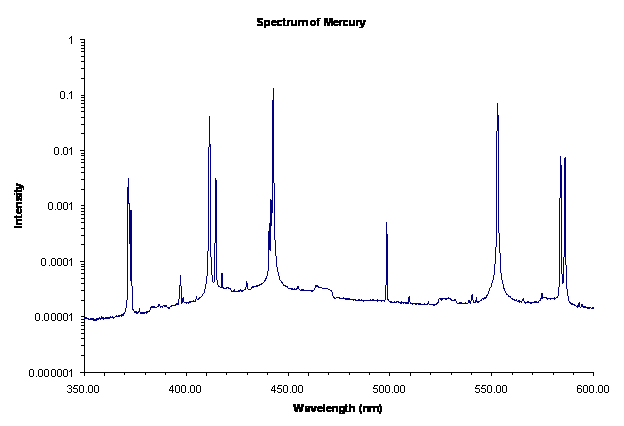
\includegraphics[width=0.8\linewidth]{images/Atmimage015.png}}
    \caption{Spectrum of Mercury}
    \label{fig:Atmimage015}
\end{figure}

\subsection{Additional Questions: Balmer Series}

\checkpoint{Additional Questions}{Discuss the following questions and answers with a GSI:}

    \begin{enumerate}

       \item \textbf{What elements in the equipment set the upper and lower limits in the wavelengths that can be observed? What are these limits?}

       \item \textbf{Calculate the dispersion and resolution of the spectrometer when it is used to observe the first order at a wavelength of 546.1 nm (mercury green line). The parameters of the spectrometer are given in the manufacturer's manual. Compare the calculated values with what you obtain experimentally.}

    \end{enumerate} 


\section{Zeeman Effect}

\subsection{Background}

Let us take a specific example of the Zeeman effect. We will draw an energy level diagram, show the splittings of the levels, show the spectral lines emitted and their polarizations when viewed perpendicular to the magnetic field. Refer to figure 1 on the following page.

At this point we need to get an idea of the magnitude of the Zeeman effect. It is derived from the following: $v \lambda = c$, energy $E = hv = hc / \lambda = hc \sigma$  where  $\sigma = 1 / \lambda$ is called the wavenumber, given in reciprocal centimeters, 1/cm or $cm^{-1}$. Because $E\propto\sigma$, it is an accepted practice to use $cm^{-1}$ as the unit of energy. An increment of energy is then $\Delta\sigma$, and the energy of Zeeman splittings is $\Delta\sigma = g m_j L B$. Here $L$ is called the Lorentz unit and is approximately 5 $\times$ 10 $^{-5}$ cm$^{-1}$/gauss. One electron volt is approximately 8000 cm$^{-1}$. [Look up all the exact numbers before you make any calculations]. For example, if we have a field of one tesla, a g-factor of 1.5, and a J-value of 2, we have a level split into 5 components, each one 0.75 cm$^{-1}$ from its neighbor. For practice, compute the separations of the Zeeman lines shown in the Figure below. You will see that the \emph{line} separations are less than the \emph{level} separations, because it is the \emph{difference} in g-factors that is important.

\begin{figure}[h]
    \centering
    \href{http://experimentationlab.berkeley.edu/sites/default/files/images/Atm1image003.gif}{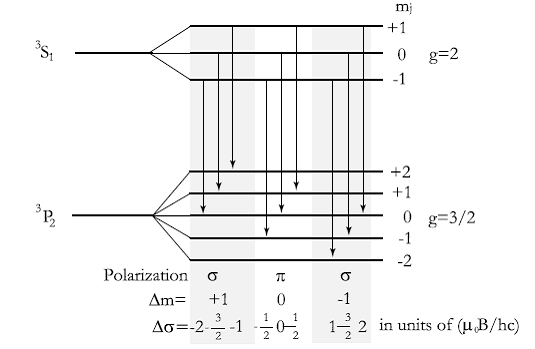
\includegraphics[width=0.5\linewidth]{images/Atm1image003.png}}
    \caption{Structure of the Zeeman multiplet \\ arising in a transition from a 3S1 to a 3P2 level.}
    \label{fig:Atm1image003}
\end{figure}

The mercury green line at 546.1 nm is an example of such a transition. [after Melissinos, p. 294]

Can we observe the Zeeman lines, in a practical case? Yes, if the lines are separated by more than their widths, and if we have a spectrometer of high enough resolution. A spectrum line has finite width (a frequency spread) because the energy levels are not infinitesimally sharp (natural width) and because the atoms are in thermal motion (Doppler width). The Doppler width is by far the larger in ordinary light sources, and has an approximate magnitude of $7 \times 10^{-7} \sigma \sqrt{T/M}$, where $T$ is the absolute temperature and $M$ is the gram atomic weight. For example, the green line of mercury at 546.1 nm in a discharge tube at room temperature has a Doppler width of 0.016 cm$^{-1}$. (Run through this calculation yourself-it will give you good practice in juggling units).

Your goals for this lab are to see the Zeeman effect in action and to learn something about the Fabry-Perot interferometer. Experimentally this is one of the easiest labs to perform, but treat it as an opportunity to learn more about the realities of quantum physics. Take the time to do a good job and to understand fully what is going on. And \emph{don't} leave your calculations and write-up until the last minute just because you think they will be easy; many students err here and receive poor grades on this easy lab just because they are rushed at the end. The same applies to presenting your oral report. There are lots of good quantum questions that can be asked.

\subsection{Apparatus}

\begin{enumerate}
    \item To observe the Zeeman effect we must put a light source in a magnetic field and observe the radiation with a spectrometer which will resolve the Zeeman lines. We are going to use a discharge tube, an ordinary electromagnet with iron pole pieces, a lens, a Fabry-Perot interferometer, and a digital camera, arranged in a configuration as shown in Figure~\ref{fig:ATMFig2}. 
    \begin{figure}[h]
        \centering
        \href{http://experimentationlab.berkeley.edu/sites/default/files/ATM/ATM-zeeman.png}{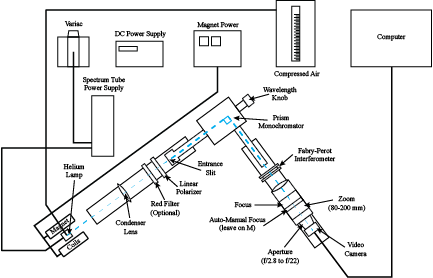
\includegraphics[width=0.5\linewidth]{images/ATM-zeeman.png}}
        \caption{Apparatus}
        \label{fig:ATMFig2}
    \end{figure}

	The lens is present merely to get light into the interferometer; it plays no part in resolving the spectrum lines. The interferometer forms fringes at infinity, as will be discussed below, and the camera is used to magnify and view these fringes. It is possible to dispense with the camera if you can focus your eyes at infinity but the fringes will look smaller and be harder to see.

    \item The Fabry-Perot interferometer (see Jenkins \& White \href{http://physics111.lib.berkeley.edu/Physics111/Reprints/ATM/04-Interference.pdf}{\textbf{``Ch. 14: Interference Involving Multiple Reflections}}''; also look at \href{http://youtu.be/zUGBt5vc5FA}{\textbf{Video Optical Instruments}}) works on the principle of multiple amplitude division of a wavefront and recombination of these wavefronts, each of which has traveled a different optical path length. We can represent these wavefronts by rays, as shown in Figure~\ref{fig:Atm1image005}.

    \begin{figure}[H]
        \centering
        \href{http://experimentationlab.berkeley.edu/sites/default/files/images/Atm1image005.gif}{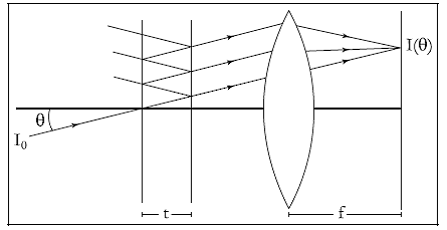
\includegraphics[width=0.5\linewidth]{images/Atm1image005.png}}
        \caption{Fabry-Perot interferometer}
        \label{fig:Atm1image005}
    \end{figure}

    The interferometer itself is nothing but two plane parallel partially-reflecting films. In our case they are multi-layer dielectric coated mirrors supported on two flat quartz discs, called plates, or substrates. The optical path difference between two adjacent rays is $\sigma=(2t)cos\theta $, and the order of interference n is this path difference divided by the wavelength. When all the rays are added together, the intensity distribution is
    \[
    \frac{I_0}{1+\frac{4R}{(1-R)^2}\sin^2\frac{\delta}{2}},
    \textrm{ where }
    \delta = 2 \pi \frac{2t \cos\theta}{\lambda}
    \]
    is the phase difference between adjacent rays, and R is the reflectance of a single coating. The interference fringes are circles. The smallest wavenumber difference (energy) that can be resolved is given by
    \[
    \delta\sigma = \frac{1}{2 t N_R},
    \textrm{ where }
    N_R = \pi \frac{\sqrt{R}}{1-R}
    \]
    There is also a wavenumber interval called the \textbf{free spectral range}, the difference in wavenumber of two spectral lines that will give a ring of exactly the same radius (fringes at the same angle theta, but differing in order by 1.) It is also approximately the reciprocal of the path difference between adjacent fringes of the same wavelength. The F-P interferometer used in this experiment is a very precise and expensive piece of equipment. Do not touch its optical surfaces or attempt to clean it-if you think it's dirty, ask the staff for assistance. The only adjustments you need make are its horizontal and vertical orientations, controlled by the two large graticulated knobs. Its spacing ``t'' is 8.11 mm, and its reflectance R is 0.90.

\end{enumerate}

\subsection{Procedure}

\begin{enumerate}
    \item Before you turn on the helium lamp, turn on the cooling air. If the lamp gets too hot it breaks. The air valve is located above the top shelf on the right side of the ATM bench-it should be adjusted so that the indicator ball is between 40 and 50 on the scale.

    \item Make sure that the black transformer is set to zero, and then turn it on.

    \item Then turn on the wooden box marked ``HIGH VOLTAGE''. Increase the voltage on the transformer until the He tube begins to glow brightly.

    \item The \href{http://physics111.lib.berkeley.edu/Physics111/Reprints/ATM/OCR\%20Burleigh\%20tech\%20memo\%20fabry\%20perots.pdf}{\textbf{Fabry-Perot}} interferometer is already adjusted. The plates are flat and parallel to a fraction of a wavelength. Also see  \href{http://physics111.lib.berkeley.edu/Physics111/Reprints/ATM/Beam\%20Shaping.pdf}{\textbf{Beam Shaping}}

    \item See how to set up the CCD camera below so that you can use the camera's image to adjust the setup in the next step.

    \item Set up the optical system shown above on the rail closest to the edge of the table, leaving out the red filter for now. Adjust the lens until you get a crisp image from the camera. Make sure that the lamp cooling air is on and watch the lamp carefully; if it gets too hot, it will melt. The image might be very dim, as well as blocked by the magnets. Move the lens wherever you need to to get as much light as possible going through the interferometer.
    
    \checkpoint{Zeeman Picture}{Show the produced image to a GSI}
    
%    \textbf{Checkpoint: Show the produced image to a GSI.}

    \item Observe, record, and explain what happens when you do the following, using your eye instead of the camera image: move the position of the lens; tilt the F-P plates; raise and lower the interferometer. Now with the camera in place: change the position of the camera; shift the camera sideways.

    \item Put in the red glass filter; adjust the system until the fringes are sharp. Turn on the magnetic field. To control it, use the LAMBDA DC POWER SUPPLY. Turn the OUTPUT VOLTAGE VDC knob to zero, and the CURRENT LIMITER IDC knob to 2 Amps. Turn on the power supply. Increase the VDC control until you see the fringes start to split. If the lamp flickers or goes out, increase the voltage on the transformer. Can you explain why this happens? The lamp is just a tube filled with He gas, and electrons are accelerated through the tube by an electric field from the high voltage. As they travel through the tube, they collide with He atoms, and excite them. When these de-excite, they emit the characteristic He lines. Now what happens when we add a transverse magnetic field? Rotate the polarizer and note the behavior of the lines. Don't be discouraged if you see fuzzy fringes and bizarre behavior. With a little experience your skill will improve until you can produce and see the proper Zeeman effects.

    %\item \textbf{Checkpoint: Make sure you can do the following/answer the following questions before calling over your GSI or Professor to sign you off: Produce Zeeman splitting by varying the field strength. Explain why the lamp dies when a high enough field is applied. Rotate the polarizer until only the sigma components are observed; increase the field strength until the fringes show equal spacing between the rings. What fraction of an order did the magnetic field shift the frequencies of the Zeeman components of the line? [1/2, 1/3, 1/4, or ?. We take one order to be the spacing between two unsplit lines -- no magnetic field.] Repeat several times, so you can make some estimate of the error in your measurements. Measure the magnetic field strength with the gaussmeter. The He discharge tube is mounted on a track so that you can slide it back out of the center region of the magnet and position the meter probe where the tube usually sits.}
    
    \checkpoint{Zeeman Splitting}{Produce Zeeman splitting by varying the field strength. Explain why the lamp dies when a high enough field is applied. Rotate the polarizer until only the sigma components are observed; increase the field strength until the fringes show equal spacings between the rings. What fraction of an order did the magnetic field shift the frequencies of the Zeeman components of the line? [1/2, 1/3, 1/4, or ?. We take one order to be the spacing between two unsplit lines -- no magnetic field.] Repeat several times, so you can make some estimate of the error in your measurements. Measure the magnetic field strength with the gaussmeter. The He discharge tube is mounted on a track so that you can slide it back out of the center region of the magnet and position the meter probe where the tube usually sits.}

    \begin{itemize}
        \item \emph{Before taking any readings with the 5180 gaussmeter,}
        \begin{itemize}
            \item 1st = Select Auto Zero. To select AUTO ZERO operation, press the ZERO pushbutton. Unit automatically returns to normal operation.
        
            \item 2nd = Select Auto Range. To select AUTO RANGE operation, press the SHIFT pushbutton followed by the RANGE pushbutton. Press the SHIFT pushbutton followed by the RANGE pushbutton to exit Auto Range mode. Manual Range.
            
            \item Also; To select MANUAL RANGE operation, press the RANGE pushbutton. Press the UP (5) and DOWN (6) arrow pushbuttons to select ranges. Press the RANGE pushbutton to return to normal operation.
            
            \item For a complete 5180 Manual See [\href{http://physics111.lib.berkeley.edu/Physics111/Equipment\_Manuals/Gaussmeter5180.pdf}{\textbf{Gaussmeter}}]. For an interactive Manual see [\href{http://physics111.lib.berkeley.edu/Physics111/Reprints/HAL/5180Manual.exe}{\textbf{5180Manual.exe}}]
            
            \item zero it by using the Zero Gauss Chamber located in the unit, and the Zero Adjust and Differential Zero Balance knobs, and then calibrate it using the 1000 gauss Probe Reference Magnet and the Calibrate and Differential Zero Balance knobs. You may have to repeat both steps several times in order to have the meter both zeroed and calibrated correctly. Make sure that you calibrate the meter on the scale that you will use to make your measurements.
            \begin{enumerate}
                \item Turn the magnet through 90 degrees, and look at the lamp through the hole in the pole piece. What is the effect of removing the polarizer?
            
                \item \textbf{Setup the CCD Camera:} After you have the Zeeman apparatus set up, you can get an even better view of the fringes (and take some snapshots for your write-up) by using the zoom lens and video camera. Attach the camera to the FireWire cable and run FireView on the PC from the Desktop. Use the drop down menu to select the Ohcilynx card. A Prosilica Digital Camera node should appear. Select the Prosilica camera and click Connect. Click OK, then click on View and then Start Acquisition. The camera should now be showing images, though they may be dark. If you need to change the brightness of the image, click on Others --$>$ Live Control, and you may change the gain and exposure from here. Temporarily remove the filter, lens, polarizer, and interferometer and line the camera up on the window in the center of the electromagnet. Then put all of the other optics back in place and align each component vertically with the aid of the camera. Zoom out all the way and set the focus to infinity. You can use the micrometer adjustment knobs on the Fabry-Perot mount to center the fringes in the field of the camera.
            
                \begin{itemize}
                    \item To take a snapshot, select Disk --$>$ Save Bitmap, and choose an appropriate location.
                \end{itemize}
            
            \end{enumerate}

        \end{itemize}
        
    \end{itemize}
    
    \begin{figure}[H]
    \centering
        \href{http://experimentationlab.berkeley.edu/sites/default/files/images/Atmimage031.gif}{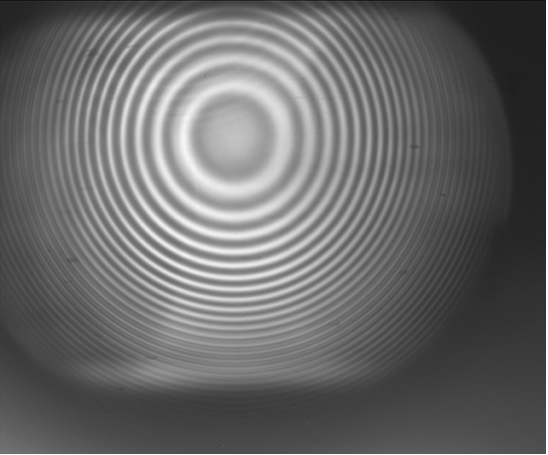
\includegraphics[width=0.6\linewidth]{images/Atmimage031.png}} \\
        \caption{Captured image from Fabry-Perot interferometer}
        \label{CapturedImage}
    \end{figure}
    
    \item \textbf{Something more complex and interesting:} Use the spectrometer to see what lines are actually present in helium. Set up the system to use the prism spectrometer as a filter to isolate the red, yellow, and blue lines, and observe the splitting with the interferometer. The trick here is to focus the light from the lamp on the slit of the prism spectrometer and open the slit up all the way to let in as much light as possible. Then closing it down to see the yellow line in the center of the eyepiece. Ensure that the lens focuses a sharp line of light onto the slit. The optical equipment should already be aligned for this, just move the lens along the track until the line is sharp. When using the camera, try using the Live Control Settings: Auto-Exposure 0, Gain 8, Shutter 425, Brightness 90, camera focal length set to infinity and zoom set to 80. If you go to edit the live controls and they are not having an effect, try restarting the computer or adjusting the lamp voltage until the rings are brighter.
    
    \begin{figure}[H]
    \centering
        \href{http://experimentationlab.berkeley.edu/sites/default/files/images/ATM_Zeeman_3489-Crop-Lg.jpg}{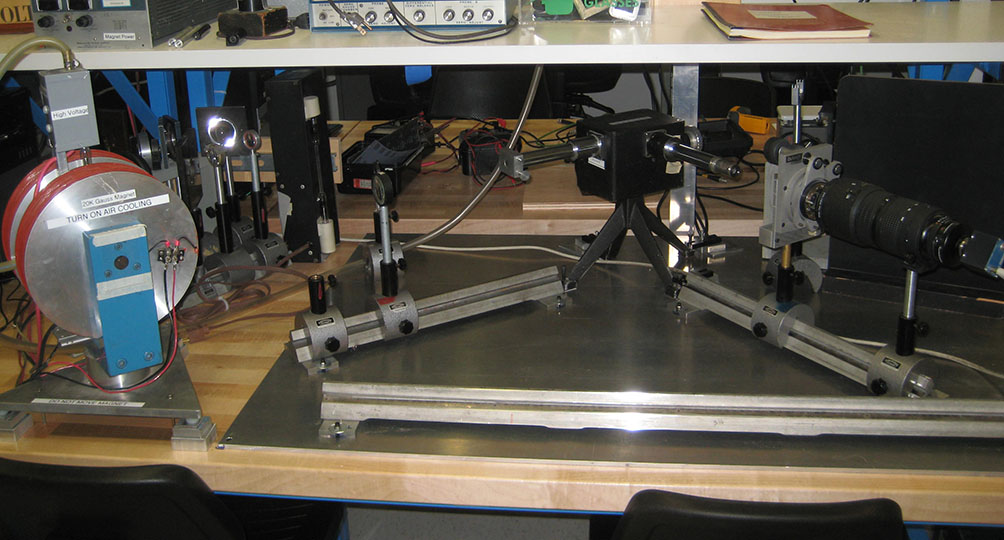
\includegraphics[width=0.8\linewidth]{images/ATM_Zeeman_3489-Crop-Lg.jpg}} \\
        \caption{Setup Using the Prism Spectrometer}
        \label{PrismSpectrometer}
    \end{figure}
    
    Find the levels which give rise to the 587.56 nm lines of helium. Work out the Zeeman pattern thoroughly enough to show you understand the problems. You will need to check out the magnitudes of the triplet splittings. Use the spectrometer together with the interferometer to observe the Zeeman effect in this line, and compare to the calculated pattern. Why don't you see a clear pattern? Can you still see polarization effects? Originally Zeeman did not have enough resolution or magnetic field to see components clearly, but only slight polarization effects in the wings of the line.

\end{enumerate}

\subsection{Calculations}

\begin{enumerate}
    \item Using your observations, calculate the ratio of energy level splitting to magnetic field, expressed in cm-1/gauss. Always use these units. While others such as joules/gauss are correct, they are never used by practicing spectroscopists. Compare to the value of the Bohr magneton based on universal constants (m, e, h, etc.). The thickness of the spacer is 8.11 mm, and its reflectance R is 0.90
\end{enumerate}

\section{Appendix}
\label{sec:Appendix}

\subsection{Acton 0.5 Meter Monochromator}

\textbf{Sections of the Operating Instructions ARC Model AM-505 Atmospheric Monochromator}

SECTION III: OPERATION

Bilateral Slit Assemblies: Slit Width: The slit width of each bilateral slit assembly is adjustable from 0.005 mm to 3 mm (5 to 3,000 microns), by a micrometer knob located on the slit housing. The knob is graduated in 0.01 millimeter (10 micron) increments. One counterclockwise revolution of the micrometer knob increases the slit width 0.25 mm (250 microns). For maximum reproducibility the slit width should be set in a counterclockwise direction (increasing slit widths) each time it is changed. The micrometer knob should not be rotated below a reading of 0.05 or above a reading of 3.00. A micrometer setting of less than 0.005 mm (5 microns) should not be used, because a stop is provided to prevent the jaws from touching each other.

Wavelength Indicator: A five-digit mechanical counter is mounted on the side of the instrument housing, and indicates the wavelength at the exit slit in Angstrom units when a 1800 G/mm grating is used. For other grating groove spacings, simply factor the counter reading in an inverse proportion to the change in groove spacing. For example, if a 300 G/mm grating is installed, the counter reading must be multiplied by six to obtain the correct wavelength at the exit slit. [***Note: the grating installed in the monochromator in 111-Lab has 300 G/mm.***].

Manual Scanning Drive: A manual scanning knob is located in the side of the instrument housing, adjacent to the Wavelength Indicator. One revolution of this knob changes the wavelength by 20 Angstroms when a 1800 G/mm grating is installed. NOTE: The speed control knob must be disengaged - placed between any two speed positions - before turning the manual scan knob. To change the speed control knob, first pull it out and then turn it. CAUTION: Do not force Manual Scanning Knob. Do not scan below a counter reading of 99990 (equivalent to $-$10), or above a counter reading of 8000.

Synchronous Motor Scanning Drive: A synchronous motor with a ten-speed transmission provides scanning speeds from 1 to 1000 Angstroms/minute. The various speeds are controlled by a speed control knob located on the side of the instrument housing. The speed control knob is labeled with the scanning speed directly in Angstroms per minute with a 1800 G/mm grating installed. For other grating groove spacings, factor the speeds in the same manner as the wavelength counter. To set the desired speed knob position, pull the speed control knob out and rotate until the desired position is in line with the dot on the instrument housing; release the knob to engage the transmission. To scan manually, set the speed control knob between any two speed positions. A scan power and direction switch is also located on the side of the instrument housing. The switch is labeled ``H'' (higher), ``OFF'' and ``L'' (lower). To scan to lower wavelengths move the scan switch to the ``L'' position, and to scan toward higher wavelengths move to the ``H'' position. Scans should be made to higher wavelengths for maximum reproducibility and accuracy.

Moveable Diverter Mirror: A moveable diverter mirror directs the beam either straight through, ``O'' position, to the PMT, or to the side slit in the ``S'' position. A knob on the top of the instrument indexes the mirror to either the ``O'' or ``S'' position. To change the mirror position, gently rotate the knob to the desired ``S'' or ``O'' position; a click will be heard and felt when the mirror indexes into position.

\begin{itemize}
    \item FOR FURTHER INFORMATION, SEE THE COMPLETE MANUAL ON THE 111-LAB Physics Library Site at [\href{http://physics111.lib.berkeley.edu/Physics111/Equipment\_Manuals/ATM\_Equipment\_Manuals/07-monochrometerAM505.pdf}{\textbf{Monochromator Manual}}]

    \item Last day of the experiment please fill out the \href{\ExperimentEvaluation}{\textbf{Experiment Evaluation}}

\end{itemize}

\section{References}
\label{sec:References}

\begin{enumerate}
    \item Herzberg, Gerhard. \emph{\href{http://physics111.lib.berkeley.edu/Physics111/Reprints/ATM/02-2ndEd-Atomic\_Spectra\_and\_Atomic\_Structure.pdf}{\textbf{Atomic Spectra \& Atomic Structure}}}, Dower Publisher, 1944, New York. Preface pg. 1-257. \#QC451.H43 (this is an old text, but gives a good perspective on how the theory developed.)

    \item Knoll Ch.9. \emph{\href{http://physics111.lib.berkeley.edu/Physics111/Reprints/Knoll-Radiation\%20Detection\%20&\%20Measurement/01-Radiation\_Detection\_and\_Measurement\_CH\_09.pdf}{\textbf{Photomulitiplier Tubes Ch.9}}}

\end{enumerate}

\noindent\textbf{Other References:}

\begin{enumerate}
    \item \emph{Introduction to Atomic Spectra,} H. E. White: (This classic text was written by one of our own faculty members, and is still useful after 65 years.)
    \begin{enumerate}
        \item \href{http://physics111.lib.berkeley.edu/Physics111/Reprints/ATM/Introduction\%20to\%20Atomic\%20Harvey\%20E.\%20White/Ch.\%201\%20early\%20historical\%20developments\%20in\%20atomic\%20spectra\_OCR.pdf}{\textbf{Ch. 1: Early Historical Developments in Atomic Spectra}},
    
        \item \href{http://physics111.lib.berkeley.edu/Physics111/Reprints/ATM/Introduction\%20to\%20Atomic\%20Harvey\%20E.\%20White/Ch.\%207\%20penetrating\%20and\%20nonpenetrating\%20orbits\%20in\%20the\%20alkali\%20metals\_OCR.pdf}{\textbf{Ch. 7: Penetrating and Non-Penetrating Orbits in the Alkali Metals}},
        
        \item \href{http://physics111.lib.berkeley.edu/Physics111/Reprints/ATM/Introduction\%20to\%20Atomic\%20Harvey\%20E.\%20White/Ch.\%208\%20doublet\%20fine\%20structure\%20and\%20the\%20spinning\%20electron\_OCR.pdf}{\textbf{Ch. 8: Doublet Fine Structure and the Spinning Electron}},
        
        \item \href{http://physics111.lib.berkeley.edu/Physics111/Reprints/ATM/Introduction\%20to\%20Atomic\%20Harvey\%20E.\%20White/Ch.\%209\%20hydrogen\%20fine\%20structure\%20and\%20the\%20dirac\%20electron\_OCR.pdf}{\textbf{Ch. 9: Hydrogen Fine Spectra and the Dirac Electron}},
        
        \item \href{http://physics111.lib.berkeley.edu/Physics111/Reprints/ATM/Introduction\%20to\%20Atomic\%20Harvey\%20E.\%20White/Ch.\%2010\%20the\%20zeeman\%20effect\%20and\%20the\%20paschen-back\%20effect\_OCR.pdf}{\textbf{Ch. 10: The Zeeman Effect and the Paschen-Back Effect}},
        
        \item \href{http://physics111.lib.berkeley.edu/Physics111/Reprints/ATM/Introduction\%20to\%20Atomic\%20Harvey\%20E.\%20White/Ch.\%2015\%20the\%20zeeman\%20effect\%20and\%20magnetic\%20quantum\%20numbers\%20in\%20complex\%20spectra\_OCR.pdf}{\textbf{Ch. 15: The Zeeman Effect and Magnetic Quantum Numbers in Complex Spectra}},
        
        \item \href{http://physics111.lib.berkeley.edu/Physics111/Reprints/ATM/Introduction\%20to\%20Atomic\%20Harvey\%20E.\%20White/Ch.\%2018\%20hyperfine\%20structure\_OCR.pdf}{\textbf{Ch. 18: Hyperfine Structure}},
    \end{enumerate}

    \item Jenkins, F.A. and White, H.E. ``\href{http://physics111.lib.berkeley.edu/Physics111/Reprints/ATM/07-Magneto-Optics\_and\_Electro-Optics.pdf}{\textbf{Ch. 32: Magneto-Optics and Electronics}}'', \emph{Fundamental of Optics}, 4th ed., 1957, pp. 679-686. \#QC356.J4..
    
    \item Melissinos, Adrian C. ``\href{http://physics111.lib.berkeley.edu/Physics111/Reprints/ATM/06-High-Resolution\_Spectroscopy.pdf}{\textbf{Ch. 7: High-Resolution Spectroscopy}}'', \emph{Experiments in Modern Physics} cp.1966; pp. 280-327. \#QC33.M4.
    
    \item Scherberger, R.F. ``\href{http://physics111.lib.berkeley.edu/Physics111/Reprints/ATM/01-Ultraviolet\_Radiation.pdf}{\textbf{Ultraviolet Radiation, Black and Otherwise}}'', Eastman Organic Chemical Bulletin: vol. 49, No. 2, 1977, pp. 1-2.
    
    \item Harnwell, G.P., and Livingood, J.J., ``\href{http://physics111.lib.berkeley.edu/Physics111/Reprints/ATM/03-Line\_Spectra.pdf}{\textbf{Ch. 7: Line Spectra}}'', \emph{Experimental Atomic Physics}, 1st edition, McGraw-Hill, pp.224-288. \#QC173.H38.
    
    \item Fowles, Grant R. ``\href{http://physics111.lib.berkeley.edu/Physics111/Reprints/ATM/05-Quantum\_Mechanics\_of\_H\_Atom.pdf}{\textbf{Ch. 7.5: Quantum Mechanics of the Hydrogen Atom}}'', \emph{Introduction to Modern Optics}, pp. 235-242. \#QC356.F65.
    
    \item Jenkins, F.A. and White, H.E. ``\href{http://physics111.lib.berkeley.edu/Physics111/Reprints/ATM/04-Interference.pdf}{\textbf{Ch. 14: Interference Involving Multiple Reflections}}'', \emph{Fundamental of Optics}, 4th ed., McGraw-Hill, 1976, pp.286-314. \#QC355.2.J461.
    
    \item \href{http://physics111.lib.berkeley.edu/Physics111/Equipment\_Manuals/RCA\_PMT.pdf}{\textbf{RCA-Photo-Multiplier-Tube-PMT-Manual}}
    
    \item \emph{Optics,} Hecht and A. Zajac:
    \begin{enumerate}
        \item \href{http://physics111.lib.berkeley.edu/Physics111/Reprints/ATM/Optics\%20Hecht\%20&\%20Zajac/Ch.\%204\%20the\%20propagation\%20of\%20light.pdf}{\textbf{Ch. 4: The Propagation of Light}},
        
        \item \href{http://physics111.lib.berkeley.edu/Physics111/Reprints/ATM/Optics\%20Hecht\%20&\%20Zajac/Ch.\%205\%20geometric\%20optics\%20--\%20paraxial\%20theory.pdf}{\textbf{Ch. 5: Geometric Optics - Paraxial Theory}},
        
        \item \href{http://physics111.lib.berkeley.edu/Physics111/Reprints/ATM/Optics\%20Hecht\%20&\%20Zajac/Ch.\%206\%20more\%20on\%20geometrical\%20optics.pdf}{\textbf{Ch. 6: More Geometrical Optics}},
        
        \item \href{http://physics111.lib.berkeley.edu/Physics111/Reprints/ATM/Optics\%20Hecht\%20&\%20Zajac/Ch.\%208\%20polarization.pdf}{\textbf{Ch. 8: Polarization}},
        
        \item \href{http://physics111.lib.berkeley.edu/Physics111/Reprints/ATM/Optics\%20Hecht\%20&\%20Zajac/Ch.\%209\%20interference.pdf}{\textbf{Ch. 9: Interference}},
        
        \item \href{http://physics111.lib.berkeley.edu/Physics111/Reprints/ATM/Optics\%20Hecht\%20&\%20Zajac/Ch.\%2010\%20diffraction.pdf}{\textbf{Ch. 10: Diffraction}},
    \end{enumerate}
    
    \item \emph{Atomic Energy Levels and Grotrian Diagrams,} Bashkin and J. M. Stoner, ``\href{http://physics111.lib.berkeley.edu/Physics111/Reprints/ATM/Atomic\%20Energy\%20Levels\%20and\%20Grotrian\%20Diagrams/atomic\%20energy\%20levels\%20-\%20hydrogen\_OCR.pdf}{\textbf{Hydrogen}}, \href{http://physics111.lib.berkeley.edu/Physics111/Reprints/ATM/Atomic\%20Energy\%20Levels\%20and\%20Grotrian\%20Diagrams/atomic\%20energy\%20levels\%20-\%20helium\_OCR.pdf}{\textbf{Helium}}, \href{http://physics111.lib.berkeley.edu/Physics111/Reprints/ATM/Atomic\%20Energy\%20Levels\%20and\%20Grotrian\%20Diagrams/atomic\%20energy\%20levels\%20-\%20potassium\_OCR.pdf}{\textbf{Potassium}}'',
    
    \item \emph{Atomic Energy Levels,} C. E. Moore (1949). ``\href{http://physics111.lib.berkeley.edu/Physics111/Reprints/ATM/Atomic\%20Energy\%20Levels/OCR\%20Hydrogen.pdf}{\textbf{Hydrogen}}, \href{http://physics111.lib.berkeley.edu/Physics111/Reprints/ATM/Atomic\%20Energy\%20Levels/OCR\%20Helium.pdf}{\textbf{Helium}}, \href{http://physics111.lib.berkeley.edu/Physics111/Reprints/ATM/Atomic\%20Energy\%20Levels/OCR\%20Potassium.pdf}{\textbf{Potassium}},'' Easiest place to find exact values of energy levels and transition energies for the red and yellow lines of helium.
    
    \item Louis Lyons, \emph{\href{http://physics111.lib.berkeley.edu/Physics111/Reprints/Data\%20Analysis\%20Book\%20PDF/Error\%20Analysis\%20Book-Louis\%20Lyons.pdf}{\textbf{A Practical Guide to Data Analysis for Physical Science Students}}}, Cambridge University Press (1994).
    
    \item Yardley Beers, \emph{\href{http://physics111.lib.berkeley.edu/Physics111/Reprints/Data\%20Analysis\%20Book\%20PDF/Error\%20Analysis\%20-\%20Beers\_Theory\%20of\%20Error.pdf}{\textbf{Introduction to the Theory of Error}}}, Addison Wesley Publishers, (1957). This is a short book which is very good.
    
    \item \href{http://experimentationlab.berkeley.edu/ATMAppendix1}{\textbf{Appendix I: ARC Model AM-505 Atmospheric Monochromator}}
\end{enumerate}

\noindent Other reprints and reference materials can be found on the \href{\LabReprints}{\textbf{Physics 111 Library Site}}

\end{document}
